\documentclass[conference]{IEEEtran}
\IEEEoverridecommandlockouts
\usepackage[T1]{fontenc}
\usepackage{cite}
\usepackage{amsmath,amssymb}
\usepackage{graphicx}
\usepackage{booktabs}
\usepackage{array}
\usepackage{url}
\usepackage[hidelinks]{hyperref}

\newif\ifanycitation
\let\citeAnyKey\cite
\renewcommand{\cite}{\global\anycitationtrue\citeAnyKey}
\let\nociteAnyKey\nocite
\renewcommand{\nocite}{\global\anycitationtrue\nociteAnyKey}

% Written by analysis/paper_numbers.py. Do not edit.
\newcommand{\AurocScratchZero}{0.9845}
\newcommand{\AurocScratchZeroLo}{0.9702}
\newcommand{\AurocScratchZeroHi}{0.9951}
\newcommand{\AccScratchZero}{0.963}
\newcommand{\AccScratchZeroLo}{0.9403}
\newcommand{\AccScratchZeroHi}{0.9830}
\newcommand{\EpochScratchZero}{82}
\newcommand{\ThrScratchZero}{0.718}
\newcommand{\AccThrScratchZero}{0.957}
\newcommand{\PInhScratchZero}{0.11}
\newcommand{\AurocScratchOne}{0.9897}
\newcommand{\AurocScratchOneLo}{0.9810}
\newcommand{\AurocScratchOneHi}{0.9965}
\newcommand{\AccScratchOne}{0.960}
\newcommand{\AccScratchOneLo}{0.9375}
\newcommand{\AccScratchOneHi}{0.9773}
\newcommand{\EpochScratchOne}{72}
\newcommand{\ThrScratchOne}{0.727}
\newcommand{\AccThrScratchOne}{0.955}
\newcommand{\PInhScratchOne}{0.11}
\newcommand{\AurocScratchTwo}{0.9651}
\newcommand{\AurocScratchTwoLo}{0.9452}
\newcommand{\AurocScratchTwoHi}{0.9803}
\newcommand{\AccScratchTwo}{0.767}
\newcommand{\AccScratchTwoLo}{0.7215}
\newcommand{\AccScratchTwoHi}{0.8069}
\newcommand{\EpochScratchTwo}{47}
\newcommand{\ThrScratchTwo}{0.986}
\newcommand{\AccThrScratchTwo}{0.909}
\newcommand{\PInhScratchTwo}{0.79}
\newcommand{\AurocScratchThree}{0.9862}
\newcommand{\AurocScratchThreeLo}{0.9756}
\newcommand{\AurocScratchThreeHi}{0.9947}
\newcommand{\AccScratchThree}{0.855}
\newcommand{\AccScratchThreeLo}{0.8153}
\newcommand{\AccScratchThreeHi}{0.8892}
\newcommand{\EpochScratchThree}{53}
\newcommand{\ThrScratchThree}{0.987}
\newcommand{\AccThrScratchThree}{0.952}
\newcommand{\PInhScratchThree}{0.54}
\newcommand{\AurocScratchFour}{0.9740}
\newcommand{\AurocScratchFourLo}{0.9582}
\newcommand{\AurocScratchFourHi}{0.9877}
\newcommand{\AccScratchFour}{0.855}
\newcommand{\AccScratchFourLo}{0.8182}
\newcommand{\AccScratchFourHi}{0.8864}
\newcommand{\EpochScratchFour}{60}
\newcommand{\ThrScratchFour}{0.986}
\newcommand{\AccThrScratchFour}{0.909}
\newcommand{\PInhScratchFour}{0.50}
\newcommand{\meanAurocScratch}{0.9799}
\newcommand{\sdAurocScratch}{0.0101}
\newcommand{\minAurocScratch}{0.9651}
\newcommand{\maxAurocScratch}{0.9897}
\newcommand{\rangeAurocScratch}{0.025}
\newcommand{\meanAccScratch}{0.8801}
\newcommand{\minAccScratch}{0.767}
\newcommand{\maxAccScratch}{0.963}
\newcommand{\halfWidthScratch}{0.012}
\newcommand{\minutesScratch}{31}
\newcommand{\paramsScratch}{33.16}
\newcommand{\AurocKineticsZero}{0.9856}
\newcommand{\AurocKineticsZeroLo}{0.9756}
\newcommand{\AurocKineticsZeroHi}{0.9940}
\newcommand{\AccKineticsZero}{0.946}
\newcommand{\AccKineticsZeroLo}{0.9233}
\newcommand{\AccKineticsZeroHi}{0.9688}
\newcommand{\EpochKineticsZero}{54}
\newcommand{\ThrKineticsZero}{0.326}
\newcommand{\AccThrKineticsZero}{0.952}
\newcommand{\PInhKineticsZero}{0.06}
\newcommand{\AurocKineticsOne}{0.9810}
\newcommand{\AurocKineticsOneLo}{0.9692}
\newcommand{\AurocKineticsOneHi}{0.9914}
\newcommand{\AccKineticsOne}{0.926}
\newcommand{\AccKineticsOneLo}{0.9006}
\newcommand{\AccKineticsOneHi}{0.9545}
\newcommand{\EpochKineticsOne}{47}
\newcommand{\ThrKineticsOne}{0.943}
\newcommand{\AccThrKineticsOne}{0.938}
\newcommand{\PInhKineticsOne}{0.26}
\newcommand{\AurocKineticsTwo}{0.9890}
\newcommand{\AurocKineticsTwoLo}{0.9798}
\newcommand{\AurocKineticsTwoHi}{0.9961}
\newcommand{\AccKineticsTwo}{0.952}
\newcommand{\AccKineticsTwoLo}{0.9290}
\newcommand{\AccKineticsTwoHi}{0.9716}
\newcommand{\EpochKineticsTwo}{54}
\newcommand{\ThrKineticsTwo}{0.982}
\newcommand{\AccThrKineticsTwo}{0.923}
\newcommand{\PInhKineticsTwo}{0.13}
\newcommand{\AurocKineticsThree}{0.9888}
\newcommand{\AurocKineticsThreeLo}{0.9776}
\newcommand{\AurocKineticsThreeHi}{0.9965}
\newcommand{\AccKineticsThree}{0.957}
\newcommand{\AccKineticsThreeLo}{0.9375}
\newcommand{\AccKineticsThreeHi}{0.9773}
\newcommand{\EpochKineticsThree}{86}
\newcommand{\ThrKineticsThree}{0.986}
\newcommand{\AccThrKineticsThree}{0.943}
\newcommand{\PInhKineticsThree}{0.10}
\newcommand{\AurocKineticsFour}{0.9912}
\newcommand{\AurocKineticsFourLo}{0.9841}
\newcommand{\AurocKineticsFourHi}{0.9969}
\newcommand{\AccKineticsFour}{0.957}
\newcommand{\AccKineticsFourLo}{0.9374}
\newcommand{\AccKineticsFourHi}{0.9801}
\newcommand{\EpochKineticsFour}{71}
\newcommand{\ThrKineticsFour}{0.458}
\newcommand{\AccThrKineticsFour}{0.952}
\newcommand{\PInhKineticsFour}{0.07}
\newcommand{\meanAurocKinetics}{0.9871}
\newcommand{\sdAurocKinetics}{0.0040}
\newcommand{\minAurocKinetics}{0.9810}
\newcommand{\maxAurocKinetics}{0.9912}
\newcommand{\rangeAurocKinetics}{0.010}
\newcommand{\meanAccKinetics}{0.9477}
\newcommand{\minAccKinetics}{0.926}
\newcommand{\maxAccKinetics}{0.957}
\newcommand{\halfWidthKinetics}{0.009}
\newcommand{\minutesKinetics}{28}
\newcommand{\paramsKinetics}{33.17}
\newcommand{\laterMeanAurocScratch}{0.9787}
\newcommand{\ValEmaScratchZero}{0.9619}
\newcommand{\ValRawScratchZero}{0.9630}
\newcommand{\ValEmaScratchOne}{0.9759}
\newcommand{\ValRawScratchOne}{0.9730}
\newcommand{\ValEmaScratchTwo}{0.9764}
\newcommand{\ValRawScratchTwo}{0.9467}
\newcommand{\ValEmaScratchThree}{0.9717}
\newcommand{\ValRawScratchThree}{0.9599}
\newcommand{\ValEmaScratchFour}{0.9585}
\newcommand{\ValRawScratchFour}{0.9552}
\newcommand{\ValEmaKineticsZero}{0.9806}
\newcommand{\ValRawKineticsZero}{0.9755}
\newcommand{\ValEmaKineticsOne}{0.9832}
\newcommand{\ValRawKineticsOne}{0.9730}
\newcommand{\ValEmaKineticsTwo}{0.9763}
\newcommand{\ValRawKineticsTwo}{0.9735}
\newcommand{\ValEmaKineticsThree}{0.9804}
\newcommand{\ValRawKineticsThree}{0.9782}
\newcommand{\ValEmaKineticsFour}{0.9790}
\newcommand{\ValRawKineticsFour}{0.9808}
\newcommand{\rhoRawTest}{0.75}
\newcommand{\rhoRawTestP}{0.013}
\newcommand{\rhoEmaTest}{0.10}
\newcommand{\maxSelectionMargin}{0.0005}
\newcommand{\rhoRawScratch}{0.90}
\newcommand{\rhoEmaScratch}{0.00}
\newcommand{\tLoScratch}{0.9673}
\newcommand{\tHiScratch}{0.9925}
\newcommand{\rhoRawKinetics}{0.70}
\newcommand{\rhoEmaKinetics}{-0.90}
\newcommand{\tLoKinetics}{0.9822}
\newcommand{\tHiKinetics}{0.9920}
\newcommand{\leveneP}{0.25}
\newcommand{\leveneMeanP}{0.034}
\newcommand{\fTestP}{0.096}
\newcommand{\probImprovement}{0.72}
\newcommand{\sdRatio}{2.6}
\newcommand{\seedDiff}{0.0072}
\newcommand{\permP}{0.20}
\newcommand{\permCount}{252}
\newcommand{\welchP}{0.20}
\newcommand{\welchDf}{5.2}
\newcommand{\welchLo}{-0.005}
\newcommand{\welchHi}{0.020}
\newcommand{\mannWhitneyP}{0.31}
\newcommand{\pairDiffZero}{0.0011}
\newcommand{\pairLoZero}{-0.0070}
\newcommand{\pairHiZero}{0.0107}
\newcommand{\pairPZero}{0.839}
\newcommand{\pairDiffOne}{-0.0087}
\newcommand{\pairLoOne}{-0.0182}
\newcommand{\pairHiOne}{-0.0002}
\newcommand{\pairPOne}{0.045}
\newcommand{\pairDiffTwo}{0.0239}
\newcommand{\pairLoTwo}{0.0097}
\newcommand{\pairHiTwo}{0.0408}
\newcommand{\pairPTwo}{<0.001}
\newcommand{\pairDiffThree}{0.0026}
\newcommand{\pairLoThree}{-0.0092}
\newcommand{\pairHiThree}{0.0147}
\newcommand{\pairPThree}{0.672}
\newcommand{\pairDiffFour}{0.0172}
\newcommand{\pairLoFour}{0.0044}
\newcommand{\pairHiFour}{0.0318}
\newcommand{\pairPFour}{0.003}
\newcommand{\pairHolmTwo}{<0.001}
\newcommand{\pairHolmFour}{0.012}
\newcommand{\pairHolmOne}{0.135}
\newcommand{\pairHolmThree}{1.000}
\newcommand{\pairHolmZero}{1.000}
\newcommand{\holmSurvive}{2}
\newcommand{\pooledDiff}{0.0072}
\newcommand{\ensembleScratch}{0.9898}
\newcommand{\ensembleKinetics}{0.9887}
\newcommand{\ensembleDiff}{-0.0011}
\newcommand{\ensembleLo}{-0.0085}
\newcommand{\ensembleHi}{0.0056}
\newcommand{\pooledLo}{-0.0009}
\newcommand{\pooledHi}{0.0155}
\newcommand{\pooledP}{0.079}
\newcommand{\pooledLoScratch}{0.9686}
\newcommand{\pooledHiScratch}{0.9895}
\newcommand{\pooledLoKinetics}{0.9780}
\newcommand{\pooledHiKinetics}{0.9943}
\newcommand{\baseTopoAuroc}{0.985}
\newcommand{\baseTopoAcc}{0.929}
\newcommand{\aboveTopoScratch}{2}
\newcommand{\ciAboveTopoScratch}{0}
\newcommand{\ciBelowTopoScratch}{1}
\newcommand{\accAboveTopoScratch}{2}
\newcommand{\aboveTopoKinetics}{4}
\newcommand{\ciAboveTopoKinetics}{0}
\newcommand{\ciBelowTopoKinetics}{0}
\newcommand{\accAboveTopoKinetics}{4}
\newcommand{\basePlaneAuroc}{0.973}
\newcommand{\basePlaneAcc}{0.930}
\newcommand{\abovePlaneScratch}{4}
\newcommand{\ciAbovePlaneScratch}{2}
\newcommand{\ciBelowPlaneScratch}{0}
\newcommand{\accAbovePlaneScratch}{2}
\newcommand{\abovePlaneKinetics}{5}
\newcommand{\ciAbovePlaneKinetics}{4}
\newcommand{\ciBelowPlaneKinetics}{0}
\newcommand{\accAbovePlaneKinetics}{4}
\newcommand{\baseParkAuroc}{0.880}
\newcommand{\baseParkAcc}{0.861}
\newcommand{\aboveParkScratch}{5}
\newcommand{\ciAboveParkScratch}{5}
\newcommand{\ciBelowParkScratch}{0}
\newcommand{\accAboveParkScratch}{2}
\newcommand{\aboveParkKinetics}{5}
\newcommand{\ciAboveParkKinetics}{5}
\newcommand{\ciBelowParkKinetics}{0}
\newcommand{\accAboveParkKinetics}{5}
\newcommand{\baseMedmnistAuroc}{0.851}
\newcommand{\baseMedmnistAcc}{0.795}
\newcommand{\aboveMedmnistScratch}{5}
\newcommand{\ciAboveMedmnistScratch}{5}
\newcommand{\ciBelowMedmnistScratch}{0}
\newcommand{\accAboveMedmnistScratch}{4}
\newcommand{\aboveMedmnistKinetics}{5}
\newcommand{\ciAboveMedmnistKinetics}{5}
\newcommand{\ciBelowMedmnistKinetics}{0}
\newcommand{\accAboveMedmnistKinetics}{5}
\newcommand{\baseMtdlAuroc}{0.951}
\newcommand{\baseMtdlAcc}{0.931}
\newcommand{\aboveMtdlScratch}{5}
\newcommand{\ciAboveMtdlScratch}{4}
\newcommand{\ciBelowMtdlScratch}{0}
\newcommand{\accAboveMtdlScratch}{2}
\newcommand{\aboveMtdlKinetics}{5}
\newcommand{\ciAboveMtdlKinetics}{5}
\newcommand{\ciBelowMtdlKinetics}{0}
\newcommand{\accAboveMtdlKinetics}{4}
\newcommand{\baseCnmtdlAuroc}{0.932}
\newcommand{\baseCnmtdlAcc}{0.855}
\newcommand{\aboveCnmtdlScratch}{5}
\newcommand{\ciAboveCnmtdlScratch}{5}
\newcommand{\ciBelowCnmtdlScratch}{0}
\newcommand{\accAboveCnmtdlScratch}{4}
\newcommand{\aboveCnmtdlKinetics}{5}
\newcommand{\ciAboveCnmtdlKinetics}{5}
\newcommand{\ciBelowCnmtdlKinetics}{0}
\newcommand{\accAboveCnmtdlKinetics}{5}
\newcommand{\oneSamplePScratch}{0.203}
\newcommand{\oneSampleTopoPScratch}{0.32}
\newcommand{\oneSamplePKinetics}{0.001}
\newcommand{\oneSampleTopoPKinetics}{0.30}
\newcommand{\dupMax}{0.25}
\newcommand{\dupMedian}{0.10}
\newcommand{\dupCount}{0}
\newcommand{\dupRef}{1407}
\newcommand{\nValExc}{129}
\newcommand{\nValInh}{48}
\newcommand{\valStep}{0.021}
\newcommand{\topoRebuiltRThreeD}{0.929}
\newcommand{\topoRebuiltMCThree}{0.943}
\newcommand{\topoRebuiltRTwoPlusOne}{0.917}
\newcommand{\gflopsScratch}{62.8}
\newcommand{\gflopsKinetics}{106.3}
\newcommand{\gflopsRatio}{1.7}
\newcommand{\nTrain}{1230}
\newcommand{\nVal}{177}
\newcommand{\nTest}{352}
\newcommand{\nTestExc}{257}
\newcommand{\nTestInh}{95}
\newcommand{\prevalence}{0.730}
\newcommand{\nSeeds}{5}
\newcommand{\replicates}{2000}
\newcommand{\bootReps}{1000}
\newcommand{\gpu}{RTX 4070 Ti}
\newcommand{\torchVersion}{2.15.0}
\newcommand{\torchvisionVersion}{0.29.2}
\newcommand{\lightningVersion}{2.6.6}
\newcommand{\monaiVersion}{1.6.2}
\newcommand{\medmnistVersion}{3.0.2}
\newcommand{\cudaVersion}{13.2}

\newcommand{\subsetsTotal}{6}
\newcommand{\subsetsAboveThen}{1}


\begin{document}

\title{Two 3D ResNet-18 Configurations Are Not Separable in Five Seeds Each on SynapseMNIST3D}

\author{
\IEEEauthorblockN{Isaiah R. Harville}
\IEEEauthorblockA{Independent Researcher}
}

\maketitle

\begin{abstract}
SynapseMNIST3D asks whether a $64^3$ electron microscopy crop shows an excitatory or an
inhibitory synapse. Its official test split holds only \nTest{} volumes, all synapses of one
neuron in one rat. None of the published results at $64^3$ that we read reports a spread in its main text. The
highest we found is \baseTopoAuroc{} AUROC, for a Kinetics-400-pretrained R3D-18 in the
TopoCAM paper, with no run count stated. We trained five seeds each of two 3D ResNet-18
configurations under one fixed, untuned recipe: a MONAI ResNet-18 from random weights and
the torchvision R3D-18 from its Kinetics-400 weights. They differ in stem, input handling,
and compute as well as in initialization. Mean test AUROC was \meanAurocScratch{} (SD
\sdAurocScratch{}) for the first and \meanAurocKinetics{} (SD \sdAurocKinetics{}) for the
second, consistent with TopoCAM's value. The difference, \seedDiff{}, is not resolved. An
exact permutation test over the ten seed values gives $p=\permP{}$, and a paired bootstrap over
test volumes puts the difference of the five-seed means between \pooledLo{} and
\pooledHi{}. The five-seed ensembles score \ensembleScratch{} and \ensembleKinetics{}. Every test number comes from the raw weights of
an epoch selected on averaged weights, so the seed spreads we measured, \minAurocScratch{}
to \maxAurocScratch{} from scratch, mix seed variation with the choice of raw snapshot and
are upper bounds. No test volume correlates
above \dupMax{} with any training or validation volume. We chose this subset after its first
result, and we release every seed's per-volume predictions.
\end{abstract}

\begin{IEEEkeywords}
SynapseMNIST3D, MedMNIST, 3D classification, electron microscopy, R3D-18, training seeds,
paired bootstrap
\end{IEEEkeywords}

\section{Introduction}

SynapseMNIST3D is one of the six 3D subsets of MedMNIST v2~\cite{yang2023medmnist}. Its
volumes are cubes cut around synapses in a multi-beam scanning electron microscopy volume of
an adult rat, all on one pyramidal neuron, labeled by experts as excitatory or inhibitory. The official split is
random, with \nTrain{} training, \nVal{} validation, and \nTest{} test
volumes~\cite{yang2023medmnist}. MedMNIST v2 reported 3D ResNets on $28^3$ inputs, with a
best AUROC of \baseMedmnistAuroc{}~\cite{yang2023medmnist}. MedMNIST+ added $64^3$
versions~\cite{yang2024medmnistplus}, and later work reported much higher values.
TopoCAM fine-tuned Kinetics-400-pretrained video networks and reported AUROC
\baseTopoAuroc{} for R3D-18~\cite{nuwagira2026topocam}. PlaneCycle reported
\basePlaneAuroc{}, a mean of five runs, for a fully fine-tuned 3D ViT-L/16, without stating
the input size~\cite{yu2026planecycle}. Neither gives a standard deviation, an interval, or
per-volume predictions.

With \nTestInh{} inhibitory test volumes, one inhibitory volume scored above every
excitatory one lowers AUROC by $1/\nTestInh{}\approx 0.011$, and the 95\% bootstrap
interval of one of our from-scratch runs reaches on average \halfWidthScratch{} on either
side of its value.
That interval treats volumes from one animal as independent, so it is likely too narrow.
Training seeds add their own spread. Bouthillier et al.\ list weight initialization, data
order, and augmentation among the sources of benchmark variance~\cite{bouthillier2021variance},
and challenge rankings in biomedical image analysis change with the test
data~\cite{maierhein2018rankings}. In MICCAI 2023 segmentation papers, intervals
reconstructed around reported means were about three times wider than the gap between the
first- and second-ranked methods~\cite{christodoulou2024confidence}. A reader cannot tell from single values whether
\baseTopoAuroc{} and \basePlaneAuroc{} differ by more than these sources produce.

Our first from-scratch run scored \AurocScratchZero{}, within 0.001 of TopoCAM's R3D-18. We
then trained four more seeds of that network and five seeds of the R3D-18 itself, under the
same recipe. Our claim is narrow. On the official test split, the two networks cannot be
told apart over five seeds each, and the R3D-18 mean is consistent with TopoCAM's value.
Because our pipeline tests raw weights from an epoch chosen on averaged weights, we report
the seed spreads as upper bounds and do not compare them with the gaps between published
values.
The paper makes three contributions:
\begin{itemize}
\item Five-seed SynapseMNIST3D test results at $64^3$ for two 3D ResNet-18 networks under
one recipe, each seed with a bootstrap interval over test volumes, released with per-volume
predictions so that later work can run a paired test against them (Section~\ref{sec:results}).
\item Paired comparisons of the two networks over the five-seed means, seed-level tests,
and a check of how far the tested raw weights depart from the averaged weights that
validation selected
(Sections~\ref{sec:networks} and~\ref{sec:dynamics}).
\item A near-duplicate check of every test volume against the training and validation
volumes in all 48 orientations (Section~\ref{sec:data}), and an account of how this subset
was chosen from six (Section~\ref{sec:selection}).
\end{itemize}

\section{Related Work}

\emph{Results at $28^3$.} MedMNIST v2 trained ResNet-18 and ResNet-50 with 2.5D, 3D, and
ACS convolutions and two AutoML systems, and reported the mean of at least three
trials~\cite{yang2023medmnist}. Later $28^3$ results include ILPOResNet-50 at
0.940~\cite{zhemchuzhnikov2024ilponet}, C-Mixer at 0.866~\cite{zheng2023complex}, a
multi-task Swin at 0.8575 $\pm$ 0.0089~\cite{schafer2024umedpt}, and others that score
lower or report accuracy only~\cite{ziller2023interpretable,li2025tropical,kuipers2023regular,lyra2026fisher}.
These start from $28^3$ volumes and are not comparable.

\emph{Results at $64^3$ and with larger inputs.} TopoCAM~\cite{nuwagira2026topocam}
fine-tuned R3D-18, MC3-18, R(2+1)D-18, and M3T from Kinetics-400
weights~\cite{tran2018closer,kay2017kinetics} for 100 epochs with Adam, and tested the
checkpoint with the best validation AUC. Its baselines paragraph gives a learning rate of
$10^{-4}$, and its method section gives $10^{-3}$ for the R3D-18 backbone, so which one
produced the R3D-18 row is not clear. It states no run count and no test-time augmentation.
On SynapseMNIST3D these reached 0.985, 0.968, 0.975, and 0.958. TopoCAM itself, which trains
a small network on Betti curves from Grad-CAM regions of the fine-tuned R3D-18, reached
0.984. Three models trained from scratch, EfficientNet3D, 3D-CCT, and 3D-ViT, reached 0.499
to 0.588~\cite{nuwagira2026topocam}, close to chance, while our from-scratch ResNet-18
reaches 0.98, so those from-scratch baselines say little about the value of
pretraining. Its Table~2 repeats some values across datasets. The
R(2+1)D-18 Adrenal3D values equal its Synapse3D values, and the Harvard OCT accuracy column
repeats the Vessel3D accuracies for most models~\cite{nuwagira2026topocam}. Its SynapseMNIST3D values are internally consistent. At our test prevalence, with
excitatory as the positive class, its Table~9 sensitivity and specificity give accuracies of
\topoRebuiltRThreeD{}, \topoRebuiltMCThree{}, and \topoRebuiltRTwoPlusOne{} for R3D-18,
MC3-18, and R(2+1)D-18, against its reported 0.929, 0.943, and
0.918~\cite{nuwagira2026topocam}.
PlaneCycle~\cite{yu2026planecycle} lifts DINOv3 2D ViTs to 3D. Its full fine-tuning results
are means of five runs without SDs, and the paper does not state the input size. The 3D ViT-L/16 baseline reached 0.973 and PlaneCycle
0.971. Park et al.~\cite{park2026axial} trained cross-plane attention on frozen MedDINOv3
slice features~\cite{li2025meddinov3} and reached 0.880. Two topological pipelines report
0.951 (mean of three seeds)~\cite{liu2026manifold} and 0.932 (mean of five
seeds)~\cite{wachira2026combinatorial}, with no SD in the main text. Table~\ref{tab:published} lists the values we
compare with.

\emph{Seed variance and transfer.} Bouthillier et al.~\cite{bouthillier2021variance}
recommend comparing training procedures over paired runs that randomize the data split as
well as the seeds, and estimate that 29 runs per method are needed to detect a probability
of improvement above 0.75. Picard~\cite{picard2021seed} scanned many seeds in computer
vision and found it easy to pick a seed far from the average. Dodge et al.~\cite{dodge2020finetuning} found that weight initialization
and data order contribute comparably to seed variance when fine-tuning a pretrained model.
We keep the official split, have five seeds per network, and use tests that need few
assumptions about the seed distribution. On two large medical imaging tasks, Raghu et al.~\cite{raghu2019transfusion}
found that ImageNet transfer gave little performance benefit, and on COCO, He et
al.~\cite{he2019rethinking} found that pretraining mainly sped up convergence. Morales-Brotons et
al.~\cite{morales2024ema} report that an EMA of the weights gives more consistent and better
calibrated predictions than the last iterate, which bears on our use of raw weights.

\begin{table}[t]
\caption{Which published SynapseMNIST3D results do we compare with? Test AUROC and accuracy (ACC) on the official split as each paper reports them; none states its ACC threshold. Size: input edge in voxels (n.s.: not stated). Runs: how many training runs the value summarizes. None reports an SD in its main text, an interval, or per-volume predictions.}
\label{tab:published}
\centering
\footnotesize
\setlength{\tabcolsep}{3pt}
\begin{tabular}{@{}lccll@{}}
\toprule
Method & Size & Runs & AUROC & ACC \\
\midrule
R3D-18, Kinetics-400~\cite{nuwagira2026topocam} & 64 & n.s. & 0.985 & 0.929 \\
ViT-L/16, DINOv3, 3D~\cite{yu2026planecycle} & n.s. & mean of 5 & 0.973 & 0.930 \\
MedDINOv3 slices, frozen~\cite{park2026axial} & 64 & n.s. & 0.880 & 0.861 \\
MTDL~\cite{liu2026manifold} & 64 & mean of 3 & 0.951 & 0.931 \\
CNMTDL~\cite{wachira2026combinatorial} & 64 & mean of 5 & 0.932 & 0.855 \\
ResNet-50 + 3D~\cite{yang2023medmnist} & 28 & mean of $\geq$3 & 0.851 & 0.795 \\
\bottomrule
\end{tabular}
\end{table}


\section{Data}
\label{sec:data}

We use the $64^3$ release of SynapseMNIST3D from MedMNIST+ (\texttt{medmnist}
3.0.2)~\cite{yang2024medmnistplus} with its official split: \nTrain{}, \nVal{}, and \nTest{}
volumes. The test split holds \nTestExc{} excitatory and \nTestInh{} inhibitory volumes, a
prevalence of \prevalence{}. Our data module checks the archive's MD5 (\texttt{43bd14eb\ldots}) against the
\texttt{medmnist} package and divides the stored intensities by 255. The pipeline checks that the three splits share no volume.

All volumes come from one rat, and the split is random over
synapses~\cite{yang2023medmnist}, so nearby synapses can fall in different splits. To check
for near copies, we z-scored every volume and computed its Pearson correlation with each of
the \dupRef{} training and validation volumes in all 48 axis flips and permutations. The
median of each test volume's highest correlation is \dupMedian{}, and the maximum is
\dupMax{}. No test volume correlates above 0.8 with any training or validation volume
(\dupCount{} of \nTest{}). Correlation does not catch every kind of overlap, such as two
crops of one synapse offset by half a cube, but it rules out exact and flipped copies.

\section{Method}
\label{sec:method}

\begin{table}[t]
\caption{How do the two networks differ? GFLOPs: one forward pass of one $64^3$ volume. Read from the installed MONAI~1.6.2 and
torchvision~0.29.2 source~\cite{monai162resnet,torchvision029video} and our configurations.}
\label{tab:setup}
\centering
\footnotesize
\setlength{\tabcolsep}{3pt}
\begin{tabular}{@{}lll@{}}
\toprule
& ResNet-18, scratch & R3D-18, Kinetics \\
\midrule
Code & MONAI \texttt{ResNet} & torchvision \texttt{r3d\_18} \\
Initial weights & random & Kinetics-400 \\
Input & 1 channel & gray repeated to 3 channels, \\
& & Kinetics mean and SD \\
Stem & $7^3$ conv, stride 1 & $3{\times}7{\times}7$ conv, stride (1,2,2) \\
Max pool & $3^3$, stride 2 & none \\
Map after stem & $64{\times}32^3$ & $64{\times}64{\times}32^2$ \\
Blocks & $[2,2,2,2]$ basic, 64 to 512 & $[2,2,2,2]$ basic, 64 to 512 \\
Parameters & \paramsScratch{} M & \paramsKinetics{} M \\
GFLOPs & \gflopsScratch{} & \gflopsKinetics{} \\
\bottomrule
\end{tabular}
\end{table}

\subsection{Networks}

Both networks are 18-layer 3D ResNets~\cite{he2016deep} with the same four stages of two
basic blocks, from 64 to 512 channels, ending in global average pooling and one output
logit. Table~\ref{tab:setup} lists how they differ. The first is MONAI's
\texttt{ResNet}~\cite{cardoso2022monai}, which follows Hara et al.~\cite{hara2018can},
trained from random weights. The second is torchvision's R3D-18~\cite{tran2018closer},
initialized from its Kinetics-400 action recognition weights
(\texttt{R3D\_18\_Weights.KINETICS400\_V1})~\cite{kay2017kinetics}, with
the volume's first axis in the role of time. Its 400-way head is
replaced by one output with PyTorch's default linear initialization. The
two differ in their stems and input handling as well as their initial weights, and R3D-18 needs \gflopsRatio{} times the
compute because it keeps the full depth after its stem, so a difference between them cannot
be credited to pretraining alone. Neither has class weighting or label smoothing.

\subsection{Training}

Both networks train with one recipe, which was fixed for the from-scratch network before
any test result and not tuned for either. Each run trains for 100 epochs with batch size 16,
binary cross-entropy, and AdamW~\cite{loshchilov2019decoupled} at learning rate $10^{-3}$
and weight decay 0.05, under cosine annealing to $10^{-6}$~\cite{loshchilov2017sgdr}, in
bf16 mixed precision. Augmentation applies, with probability 0.8, a random affine transform
with rotations up to 0.17~rad about each axis, scaling up to 10\%, and translation up to 4
voxels, with trilinear interpolation and border padding, followed by a random flip along each axis with probability 0.5. At validation and test time, the probability is the mean over the volume and its mirror
along the last axis. The from-scratch network gets no input normalization beyond the
division by 255.

We keep an exponential moving average (EMA) of the weights and normalization buffers, a
variant of iterate averaging~\cite{polyak1992averaging}, with decay 0.9987. Lightning's \texttt{EMAWeightAveraging} callback swaps the averaged weights in
for each validation pass, so the per-epoch validation AUROC, and with it the selected epoch,
used the EMA weights. The callback writes the averaged weights only from its checkpoint save
hook, which Lightning~2.6.6 skips when the checkpoint holds weights
only~\cite{lightning266checkpoint}, as ours does. Every test number in this paper therefore
comes from the raw weights at the end of the selected epoch.

The ten runs differ only in the network and in \texttt{seed\_everything} (0 to 4), which
seeds the random initial weights (the head of R3D-18, every layer of the from-scratch
network) and the random draws of training, such as data order and augmentation. The
R3D-18 input repeats the gray channel three times and normalizes it with the Kinetics mean
(0.432, 0.395, 0.376) and SD (0.228, 0.221, 0.217). The analysis script checks that the
resolved configurations agree apart from these, that every run trained from a clean tree,
and that all ran with the same library versions on one GPU. The runs trained at five
commits, and the seed-0 from-scratch configuration lacks two later options whose defaults
are off. The code between the commits changed only a loss option for multiclass tasks, the
video network class, and code for serving and provenance.

\section{Evaluation Protocol}
\label{sec:protocol}

AUROC is the binary AUROC of the excitatory score, and ACC is accuracy with a score above
0.5 counted excitatory. Both follow the \texttt{medmnist} evaluator~\cite{medmnist2024evaluator}.
The analysis script recomputes every metric from the committed predictions, checks it
against each run's \path{metrics.json} to $10^{-9}$, and checks AUROC and ACC against the
evaluator's \texttt{getAUC} and \texttt{getACC}. Each checkpoint is the epoch with the
highest validation AUROC on \nVal{} volumes (\nValExc{} excitatory, \nValInh{} inhibitory),
where one inhibitory volume ranked above every excitatory one moves AUROC by
\valStep{}. On the averaged weights, the selected epoch beats the next-best epoch of its run
by at most \maxSelectionMargin{}. The test split was
scored once per run, after training.

Each run's interval is a 95\% percentile bootstrap~\cite{efron1979bootstrap} over test
volumes with \bootReps{} replicates. MedMNIST carries no animal or synapse-group identifier
beyond the one rat, so the bootstrap treats volumes as independent. These intervals cover
test sampling only.

We compare the two networks three ways. First, for each seed, \texttt{opendiagnostics
compare} resamples the test volumes \replicates{} times, scores both runs on each resample,
and reports the percentile interval of the AUROC difference and a two-sided $p$ at zero.
Pairing by seed carries no meaning beyond the shared seed setting. Second, the same paired
bootstrap scores the mean AUROC of each network's five seeds on each resample. This holds
the five training runs fixed and asks whether the difference of their means survives test
sampling. We report each per-seed $p$ with its Holm-adjusted value over the five
seeds, as a description only, since another pairing of the seeds would give other results. Third, seed-level tests treat the ten AUROCs as draws over training seeds on the
fixed test set: an exact permutation test of the difference in means over all
\permCount{} ways to split the ten values into two groups of five, Welch's $t$-test, and the
Mann-Whitney $U$ test. We treat the permutation test and the paired bootstrap of the
five-seed means as primary and the rest as checks. We compare the two networks' seed spreads with the median-centred Levene (Brown-Forsythe)
test, the SciPy default, and report the mean-centred Levene and $F$ tests beside it. We also
give the probability of improvement, the share of the 25 seed pairs in which R3D-18 scores
higher~\cite{bouthillier2021variance}, and the AUROC of each network's five-seed mean
probability.

The published values come with no SD, interval, or predictions, so no test against them is
possible. We report how many of our seeds and of our per-seed intervals lie above each, and
treat that as a description, not a test.

\section{Results}
\label{sec:results}

\begin{table*}[t]
\caption{Do the two networks differ on each seed? Test AUROC with its 95\% bootstrap interval over the 352 test volumes, accuracy at the 0.5 threshold (ACC), and the paired difference R3D-18 minus ResNet-18 from \texttt{opendiagnostics compare} (2000 paired replicates) with its two-sided $p$ and the Holm-adjusted $p$ over the five seeds. Runs are paired by seed number only; each test is paired over the test volumes.}
\label{tab:seeds}
\centering
\footnotesize
\setlength{\tabcolsep}{3pt}
\begin{tabular}{@{}clllllll@{}}
\toprule
Seed & ResNet-18, scratch & ACC & R3D-18, Kinetics & ACC & Difference [95\% CI] & $p$ & Holm \\
\midrule
0 & 0.9845 [0.9702, 0.9951] & 0.963 & 0.9856 [0.9756, 0.9940] & 0.946 & +0.0011 [-0.0070, +0.0107] & 0.839 & 1.000 \\
1 & 0.9897 [0.9810, 0.9965] & 0.960 & 0.9810 [0.9692, 0.9914] & 0.926 & -0.0087 [-0.0182, -0.0002] & 0.045 & 0.135 \\
2 & 0.9651 [0.9452, 0.9803] & 0.767 & 0.9890 [0.9798, 0.9961] & 0.952 & +0.0239 [+0.0097, +0.0408] & $<$0.001 & $<$0.001 \\
3 & 0.9862 [0.9756, 0.9947] & 0.855 & 0.9888 [0.9776, 0.9965] & 0.957 & +0.0026 [-0.0092, +0.0147] & 0.672 & 1.000 \\
4 & 0.9740 [0.9582, 0.9877] & 0.855 & 0.9912 [0.9841, 0.9969] & 0.957 & +0.0172 [+0.0044, +0.0318] & 0.003 & 0.012 \\
\bottomrule
\end{tabular}
\end{table*}


\begin{figure}[t]
\centering
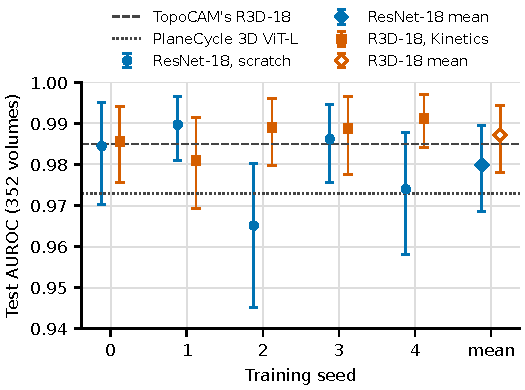
\includegraphics[width=\columnwidth]{figures/seeds.pdf}
\caption{Do the two networks' seeds separate, and where do the published values fall? Test
AUROC per seed with its 95\% bootstrap interval over the \nTest{} test volumes. Diamonds:
five-seed means with their paired-bootstrap intervals (filled: ResNet-18, open: R3D-18). Lines: TopoCAM's R3D-18 value, run
count not stated~\cite{nuwagira2026topocam}, and PlaneCycle's 3D ViT-L/16, a mean of five
runs at an unstated input size~\cite{yu2026planecycle}.}
\label{fig:seeds}
\end{figure}

\subsection{The two networks}
\label{sec:networks}

Table~\ref{tab:seeds} and Fig.~\ref{fig:seeds} give each run. The from-scratch ResNet-18
scored a mean test AUROC of \meanAurocScratch{} (SD \sdAurocScratch{}, range
\minAurocScratch{} to \maxAurocScratch{}). The Kinetics R3D-18 scored \meanAurocKinetics{}
(SD \sdAurocKinetics{}, range \minAurocKinetics{} to \maxAurocKinetics{}). The difference of
means is \seedDiff{}.

The tests do not resolve it. The exact permutation test gives $p=\permP{}$, Welch's test
$p=\welchP{}$ with \welchDf{} degrees of freedom and a 95\% interval for the difference of
\welchLo{} to \welchHi{}, and the Mann-Whitney test $p=\mannWhitneyP{}$. The paired
bootstrap of the five-seed means gives \pooledDiff{} [\pooledLo{}, \pooledHi{}],
$p=\pooledP{}$. R3D-18 scores higher in \probImprovement{} of the 25 seed pairs. The five-seed ensembles
score \ensembleScratch{} and \ensembleKinetics{}, a paired difference of \ensembleDiff{}
[\ensembleLo{}, \ensembleHi{}], so averaging seeds removes the from-scratch deficit. Table~\ref{tab:seeds}
also gives per-seed paired tests by seed number. These data are consistent with no difference, with a
ResNet-18 advantage of up to 0.005, and with an R3D-18 advantage of up to 0.02.

The from-scratch SD is \sdRatio{} times the R3D-18 SD, and the lowest from-scratch seed,
\AurocScratchTwo{}, is the only run whose interval lies wholly below \baseTopoAuroc{}.
The tests of spread disagree: the median-centred Levene test gives $p=\leveneP{}$, the
mean-centred one $p=\leveneMeanP{}$, and the $F$ test $p=\fTestP{}$. We did not choose among
them before seeing the data, so we treat the difference in spread as not established.
Section~\ref{sec:dynamics} shows that part of the from-scratch spread may come from the
weights we tested.

\subsection{Against published values}
\label{sec:published}

The R3D-18 mean, \meanAurocKinetics{}, is consistent with TopoCAM's \baseTopoAuroc{} for
the same network~\cite{nuwagira2026topocam}. The two setups differ in optimizer, learning
rate (ours $10^{-3}$, theirs $10^{-3}$ or $10^{-4}$), loss, our flip averaging, and
augmentation, which TopoCAM does not describe. Of our five R3D-18 seeds, \aboveTopoKinetics{} score above \baseTopoAuroc{}, and
every one of their intervals contains it. The 95\% $t$-interval of the R3D-18 mean, \tLoKinetics{} to \tHiKinetics{}, contains
\baseTopoAuroc{}. This fails to reject equality but does not show it.

All five R3D-18 seeds score above PlaneCycle's \basePlaneAuroc{}, and of their five
intervals, \ciAbovePlaneKinetics{} lie above it. Of the five from-scratch seeds,
\abovePlaneScratch{} score above it, and so do \ciAbovePlaneScratch{} of their intervals.
PlaneCycle's value is a mean of five runs on the same test volumes, with its own seed spread
and test-sampling error, at an input size it does not state, and it reports no SD, so we
draw no conclusion about the ordering
of the two methods. Every run of both networks, and every interval, lies above Park et
al.'s \baseParkAuroc{}~\cite{park2026axial}, CNMTDL's
\baseCnmtdlAuroc{}~\cite{wachira2026combinatorial}, and the MedMNIST v2 $28^3$ values. Every
run also scores above MTDL's \baseMtdlAuroc{}~\cite{liu2026manifold}, and every interval
lies above it except that of from-scratch seed 2.

TopoCAM's R3D-18 and MC3-18 differ by 0.017, and its R3D-18 and R(2+1)D-18 by 0.010. Our
seed ranges, \rangeAurocScratch{} and \rangeAurocKinetics{}, are of the same size, but they
are upper bounds on seed variation (Section~\ref{sec:dynamics}), so we draw no conclusion
about whether TopoCAM's ordering would survive more seeds. That needs five seeds each of
MC3-18 and R(2+1)D-18 scored on averaged weights, which we did not run.

\subsection{Accuracy at 0.5 and calibration}

Mean ACC was \meanAccScratch{} for the from-scratch network and \meanAccKinetics{} for
R3D-18. The from-scratch values split in two: \AccScratchZero{} and \AccScratchOne{} for
seeds 0 and 1, and \AccScratchTwo{}, \AccScratchThree{}, and \AccScratchFour{} for seeds 2 to
4. Those three runs selected epochs \EpochScratchTwo{}, \EpochScratchThree{}, and
\EpochScratchFour{}, when the learning rate was still high, and their raw weights give the
inhibitory test volumes mean scores of \PInhScratchTwo{}, \PInhScratchThree{}, and
\PInhScratchFour{}, against \PInhScratchZero{} for seed 0. The scores still rank most
excitatory volumes above most inhibitory ones, so AUROC holds while ACC at 0.5 falls. Their validation thresholds from Youden's index were
\ThrScratchTwo{}, \ThrScratchThree{}, and \ThrScratchFour{}, and at those thresholds
their test accuracy is \AccThrScratchTwo{}, \AccThrScratchThree{}, and
\AccThrScratchFour{}. Under the benchmark's fixed 0.5 threshold,
\accAboveTopoKinetics{} of five R3D-18 seeds and \accAboveTopoScratch{} of five
from-scratch seeds score above TopoCAM's ACC of \baseTopoAcc{}. We have not tested the EMA
weights that validation scored.

\subsection{Training dynamics and the tested weights}
\label{sec:dynamics}

\begin{figure*}[t]
\centering
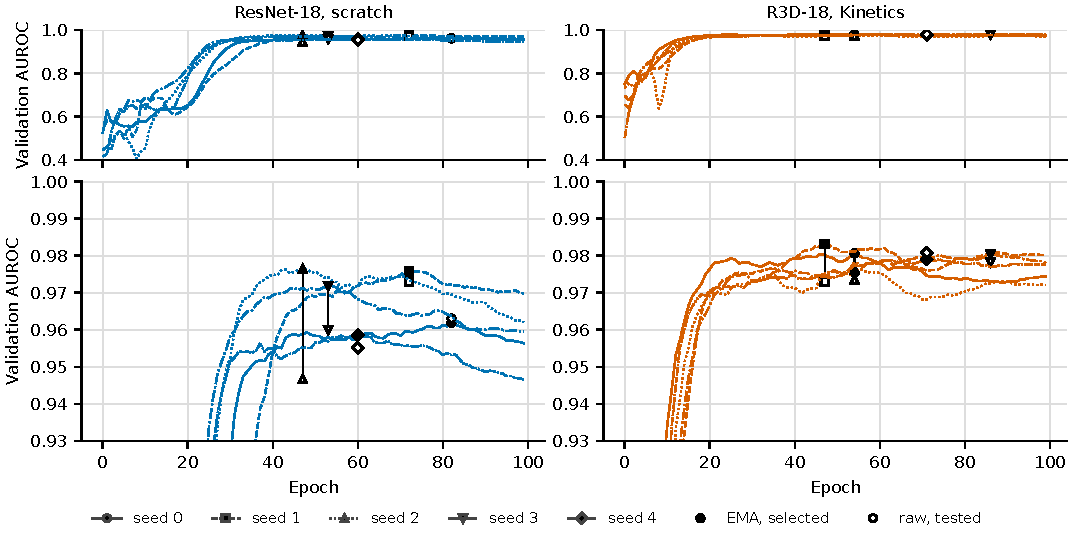
\includegraphics[width=\textwidth]{figures/training_curves.pdf}
\caption{How fast does each network reach its validation plateau, and do the tested
weights score like the selected ones? Lines: validation AUROC per epoch on the \nVal{}
validation volumes, on the EMA weights as logged during training. Filled markers: the selected epoch of each run on those weights. Open markers: the raw
weights of that epoch, which were tested. Marker shape gives the seed.
Bottom row: the same curves from 0.93 up.}
\label{fig:curves}
\end{figure*}

Fig.~\ref{fig:curves} shows validation AUROC per epoch. The R3D-18 runs pass 0.95 within
about 15 epochs. The from-scratch runs stay near 0.6 for about 20 epochs, then rise and
level off after about 35. On the EMA weights both level off between about 0.95 and 0.98, and
the selected epoch ranged from \EpochKineticsOne{} to \EpochKineticsThree{} for R3D-18 and
from \EpochScratchTwo{} to \EpochScratchZero{} for the from-scratch network.

The raw weights that were tested do not always score like the EMA weights that were
selected. For from-scratch seed 2, validation AUROC is \ValEmaScratchTwo{} on the EMA weights
and \ValRawScratchTwo{} on the raw weights, and seed 2 is our lowest test run. Within the from-scratch runs, raw-weight validation AUROC ranks test AUROC with Spearman
$\rho=\rhoRawScratch{}$, and EMA validation AUROC with $\rho=\rhoEmaScratch{}$. Within the
R3D-18 runs the values are \rhoRawKinetics{} and \rhoEmaKinetics{}, and across all ten runs
\rhoRawTest{} ($p=\rhoRawTestP{}$) and \rhoEmaTest{}. With five runs per network these are
rough, but they point one way. Because the selected epoch wins by at most
\maxSelectionMargin{} on the averaged weights, which raw snapshot gets tested is close to a
random draw from the plateau, and our seed spreads include that draw. We report them as
upper bounds on seed variation. Testing the EMA weights would settle this. Each run took about half an hour on one GPU (\minutesScratch{} and
\minutesKinetics{} minutes on average). The ensemble AUROCs in Section~\ref{sec:networks}
point the same way: the per-seed deficit of the from-scratch network disappears when its
seeds are averaged.

\subsection{How SynapseMNIST3D was chosen}
\label{sec:selection}

\begin{table*}[t]
\caption{How did the first SynapseMNIST3D run compare with the other MedMNIST 3D subsets? Test AUROC [95\% CI] of the first run of the same from-scratch ResNet-18 recipe on each subset at 64 voxels, against the best published value in that project's list when SynapseMNIST3D was chosen (commit 39e65a0) and now. Only the SynapseMNIST3D list has had a literature review since. Our CI: whether our interval lies above or below that value, or contains it.}
\label{tab:subsets}
\centering
\footnotesize
\setlength{\tabcolsep}{3pt}
\begin{tabular}{@{}llllll@{}}
\toprule
Subset & Ours [95\% CI] & Then & Our CI & Now & Our CI \\
\midrule
AdrenalMNIST3D & 0.939 [0.910, 0.963] & 0.920 & inside & 0.920 & inside \\
FractureMNIST3D & 0.781 [0.735, 0.823] & 0.750 & inside & 0.750 & inside \\
NoduleMNIST3D & 0.920 [0.878, 0.955] & 0.914 & inside & 0.914 & inside \\
OrganMNIST3D & 0.999 [0.998, 0.999] & 0.999 & inside & 0.999 & inside \\
SynapseMNIST3D & 0.984 [0.970, 0.995] & 0.880 & above & 0.985 & inside \\
VesselMNIST3D & 0.950 [0.902, 0.984] & 0.933 & inside & 0.933 & inside \\
\bottomrule
\end{tabular}
\end{table*}


The from-scratch recipe was run once on each of the six MedMNIST 3D subsets.
Table~\ref{tab:subsets} sets each first run against the best published value in that
project's list, as it stood when we chose this subset and as it stands now. At the time,
the whole interval lay above the best listed value on \subsetsAboveThen{} of
\subsetsTotal{} subsets, SynapseMNIST3D, against Park et al.'s 0.880. We chose it for that reason. The ``then'' column is the best value we had found at the
time, before the literature review. The literature review that followed found TopoCAM and PlaneCycle, and the
comparison became the one in this paper. Every later run was trained after the choice. The
four later from-scratch seeds have a mean of \laterMeanAurocScratch{}, close to the
five-seed mean, so the first seed was not far above the others. The other five lists had
no literature review, and higher published values may exist for them.

\section{Limitations}
\label{sec:limits}

Five seeds per network leave the comparison open, and the two configurations were not tuned,
so the result says nothing about either network at its best. The Welch interval allows an R3D-18
advantage of up to \welchHi{}, and the seed spreads cannot be compared with confidence. The two networks differ in stem, pooling, input handling,
and initial weights at once, and we ran no R3D-18 from random weights, so pretraining cannot
be credited or ruled out. Both networks used the from-scratch recipe, and a fine-tuning
learning rate might help the pretrained one. Test numbers come from raw weights while
selection used EMA weights, which may widen the from-scratch spread. We did not train
TopoCAM's other video networks, so we cannot say whether their published order survives
more seeds. The published baselines report no spread, so no test against them is possible,
TopoCAM's table repeats some values across datasets, and PlaneCycle's input size is not
stated. All volumes are synapses of one neuron in one rat, imaged with one microscope, the bootstrap treats volumes as independent, which likely makes our intervals too narrow, and the
near-duplicate check catches copies but not partly overlapping crops. We chose the subset
after its first result. The runs used bf16 on a GPU with nondeterministic kernels allowed,
so a rerun may not match bit for bit. This is a research result on a public benchmark and
says nothing about other animals, microscopes, or resolutions.

\section{Reproducibility and Licensing}
\label{sec:repro}

The code is at\\
\url{https://github.com/isaiah-harville/opendiagnostics}. Each run trained from a clean
tree at the commit in its \path{run.json} with one of these commands, adding
\texttt{-{}-seed\_everything=}$s$ for seeds 1 to 4.
\begin{flushleft}\footnotesize\ttfamily
uv run opendiagnostics fit -c\\
\quad models/synapsemnist3d-resnet18/config.yaml\\
uv run opendiagnostics fit -c\\
\quad models/synapsemnist3d-r3d18/config.yaml
\end{flushleft}
Training used one NVIDIA GeForce \gpu{} under Windows 11, PyTorch
\torchVersion{}~\cite{paszke2019pytorch} with CUDA \cudaVersion{}, torchvision
\torchvisionVersion{}, Lightning \lightningVersion{}~\cite{falcon2020lightning}, MONAI
\monaiVersion{}~\cite{cardoso2022monai}, and \texttt{medmnist} \medmnistVersion{}. Each run
folder under \path{models/synapsemnist3d-resnet18/runs/} and
\path{models/synapsemnist3d-r3d18/runs/} holds the resolved configuration, run record,
per-epoch history, split membership, metrics, and per-volume validation and test
predictions. The seed-0 from-scratch checkpoint is public at the URL in its
\path{artifacts.yaml}. The other nine are recorded there by SHA-256 but not uploaded. Every
number, table, and figure comes from the scripts in \path{papers/synapsemnist3d/}, which
recompute the numbers from the committed predictions with scikit-learn~\cite{pedregosa2011sklearn}
and fail on any disagreement. The figures use matplotlib~\cite{hunter2007matplotlib}.

MedMNIST releases SynapseMNIST3D under CC BY 4.0, as the run records note, which permits
redistribution with attribution, so we publish predictions and a few example test volumes.

\section{Conclusion}

Over five seeds each, a 3D ResNet-18 trained from random
weights and a Kinetics-400 R3D-18, trained with one untuned recipe and tested on raw weights, reached mean SynapseMNIST3D test AUROCs of
\meanAurocScratch{} and \meanAurocKinetics{}. The R3D-18 mean is consistent with TopoCAM's
value for that network. Paired and seed-level tests do not resolve the difference between
the two networks. The seed ensembles of the two networks differ by \ensembleDiff{}. The seed spreads,
\rangeAurocScratch{} and \rangeAurocKinetics{}, include the choice of raw snapshot and are
upper bounds. The next runs are both networks scored with the
EMA weights, an R3D-18 from random weights, a lower learning rate for the pretrained network,
and about twenty seeds per network.

\section*{Acknowledgment}

Claude, an AI model developed by Anthropic, took part in this work. It helped design and
run the experiments, wrote the analysis scripts, reviewed the literature, generated the
figures and tables, and drafted and revised the text. Isaiah R. Harville directed the
work, reviewed it, and is responsible for its content. We thank the MedMNIST team for
releasing SynapseMNIST3D under an open license.

\ifanycitation
\bibliographystyle{IEEEtran}
\bibliography{references,manual}
\fi

\end{document}
